\documentclass{article}
\usepackage[utf8]{inputenc}
\usepackage{graphicx}
\usepackage{float}
\usepackage{amsmath}
\usepackage[brazil]{babel}
\begin{document}

\title{Trabalho Avaliação de Desempenho}
\author{Eduardo Rottschaefer Oliveira \\ Universidade Federal Fluminense}
\date{\today}


\maketitle

\section{Introdução}
Este trabalho apresenta a modelagem e análise de quatro sistemas de filas utilizando a ferramenta Java Modelling Tools (JMT). Foram desenvolvidos modelos clássicos de Teoria de Filas e comparados os resultados analíticos com os resultados obtidos por simulação.

\section{Resultados}

\subsection{Modelo 1}
\subsubsection{Topologia}
\begin{figure}[H]
    \centering
    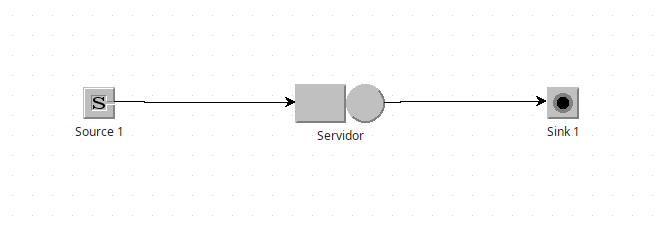
\includegraphics[width=0.8\textwidth]{topologias/modelo1.png}
    \caption{Topologia do Modelo 1}
    \label{fig:modelo1}
\end{figure}

\subsubsection{Solução Analítica}

O Modelo 1 corresponde a um sistema de filas M/M/1, composto por um único servidor, chegadas segundo um Processo de Poisson e tempos de serviço exponencialmente distribuídos.

Temos como dados de entrada:

\[
\lambda = 2 \text{ clientes/u.t.}
\]

\[
E[X] = 0.25 \text{ u.t.}
\]


O tempo médio que cada cliente passa no sistema é calculado por:

\[
E[W] = \frac{E[X]}{1-\lambda\cdot E[X]} = 0.5 \text{ u.t}
\]

O número médio de clientes no sistema é calculado por:

\[
L = {E[W]}\cdot{\lambda} = 1 \text{ cliente}
\]

O tempo médio de espera na fila pode ser obtido pela equação:

\[
E[W_Q] = E[W] - E[X] = 0.25 \text{ u.t.}
\]

\subsubsection{Resultados da Simulação}

\begin{table}[H]
    \centering
    \begin{tabular}{|l|c|c|}
        \hline
        \textbf{Medida} & \textbf{Valor}\\
        \hline
        E[W] & 0.5023682015753331 \\
        \hline
        L & 1.0057949821148777\\
        \hline
        $E[W_Q]$ & 0.24890073361364587\\
        \hline
    \end{tabular}
    \caption{Resultados da simulação para o Modelo 1}
    \label{tab:simulacao-modelo1}
\end{table}


\subsubsection{Tabela Comparativa}
% % Inserir aqui a tabela com a comparação dos resultados analíticos e simulados para o Modelo 1

\begin{table}[H]
    \centering
    \begin{tabular}{|l|c|c|c|}
        \hline
        \textbf{Medida} & \textbf{Valor teórico} & \textbf{Valor simulado} & \textbf{Diferença (\%)} \\
        \hline
        $E[W]$ & 0.5 & 0.5023682015753331 & 0.4736403 \\
        \hline
        $L$ & 1.0 & 1.0057949821148777 & 0.5795 \\
        \hline
        $E[W_Q]$ & 0.25 & 0.24890073361364587 & 0.4397 \\
        \hline
    \end{tabular}
    \caption{Tabela comparativa entre os valores teóricos e simulados para o Modelo 1}
    \label{tab:comparacao-modelo1}
\end{table}

\noindent Diferença percentual calculada por $\left|\frac{\text{simulado} - \text{teórico}}{\text{teórico}}\right| \times 100$.

\subsection{Modelo 2}
\subsubsection{Topologia}
\begin{figure}[H]
    \centering
    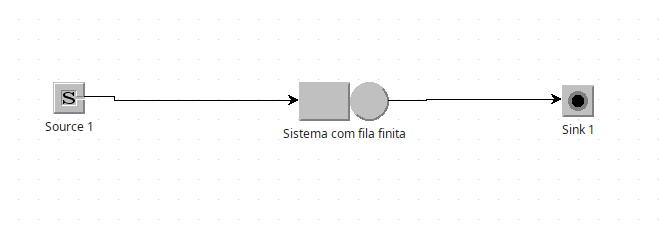
\includegraphics[width=0.8\textwidth]{topologias/modelo2.png}
    \caption{Topologia do Modelo 2}
    \label{fig:modelo2}
\end{figure}

\subsubsection{Solução Analítica}
O Modelo 2 corresponde a um sistema de filas M/M/1/b, composto por um único servidor, chegadas segundo um Processo de Poisson, tempos de serviço exponencialmente distribuídos e fila finita.

Temos como dados de entrada:

\[
\lambda = 2 \text{ clientes/u.t.}
\]

\[
\mu \approx 2.86 \text{ clientes/u.t.}
\]

\[
{b} = 10 \text{ clientes}
\]

\[
\rho = \frac{\lambda}{\mu} = 0.7
\]


O número médio de clientes no sistema é calculado por:

\begin{equation}
L =
\frac{\lambda \left(1 + b\rho^{\,b+1} - (b+1)\rho^{\,b}\right)}
{(\mu-\lambda)\left(1-\rho^{\,b+1}\right)} \approx 2.10 
\end{equation}

O tempo médio que cada cliente passa no sistema, desconsiderando os que chegam e encontram a fila cheia, pode ser obtido pela equação:

\[
E[W] = \frac{L}{\lambda_a}
\]

Onde: 

\[
\lambda_a = \lambda \left(1-\pi_b\right) \approx 1.98
\]

Logo:

\[
E[W] \approx 1.06 \text{ u.t}
\]


\subsubsection{Resultados da Simulação}

\begin{table}[H]
    \centering
    \begin{tabular}{|l|c|c|}
        \hline
        \textbf{Medida} & \textbf{Valor}\\
        \hline
        L & 2.1223516367762114 \\
        \hline
        E[W] & 1.0679721686761363\\
        \hline
        $E[W_Q]$ & 0.7116977904499656\\
        \hline
        $\textit{Drop Rate} $ &  0.017412819279805602\\
        \hline
    \end{tabular}
    \caption{Resultados da simulação para o Modelo 2}
    \label{tab:simulacao-modelo2}
\end{table}
\subsubsection{Tabela Comparativa}

\begin{table}[H]
    \centering
    \begin{tabular}{|l|c|c|c|}
        \hline
        \textbf{Medida} & \textbf{Valor teórico} & \textbf{Valor simulado} & \textbf{Diferença (\%)} \\
        \hline
        $L$ & 2.10 & 2.1223516367762111 & 1.0643637 \\
        \hline
        $E[W]$ & 1.06 & 1.0679721686761363 & 0.7520914 \\
        \hline
    \end{tabular}
    \caption{Tabela comparativa entre os valores teóricos e simulados para o Modelo 2}
    \label{tab:comparacao-modelo2}
\end{table}

\subsection{Modelo 3}
\subsubsection{Topologia}
\begin{figure}[H]
    \centering
    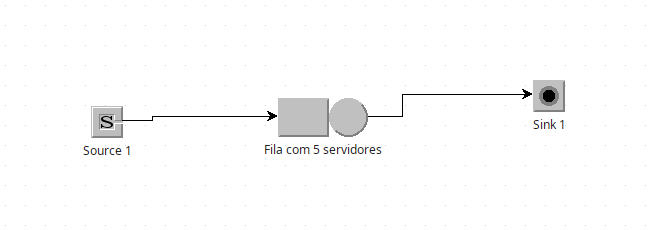
\includegraphics[width=0.8\textwidth]{topologias/modelo3.png}
    \caption{Topologia do Modelo 3}
    \label{fig:modelo3}
\end{figure}

\subsubsection{Resultados da Simulação}

\begin{table}[H]
    \centering
    \begin{tabular}{|l|c|c|}
        \hline
        \textbf{Medida} & \textbf{Valor}\\
        \hline
        L & 6.1425309496845095 \\
        \hline
        E[W] & 1.5467049099965863\\
        \hline
        $E[W_Q]$ & 0.5501108205969217\\
        \hline

    \end{tabular}
    \caption{Resultados da simulação para o Modelo 3}
    \label{tab:simulacao-modelo3}
\end{table}

\subsection{Modelo 4}

\subsubsection{Topologia}
\begin{figure}[H]
    \centering
    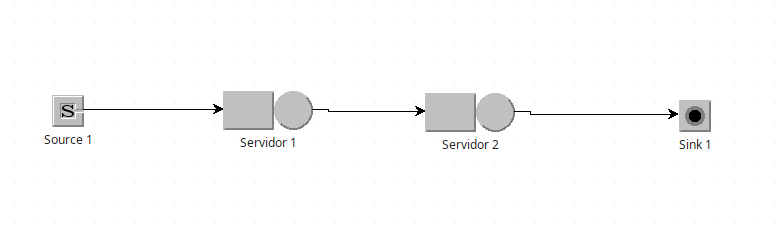
\includegraphics[width=0.8\textwidth]{topologias/modelo4.png}
    \caption{Topologia do Modelo 4}
    \label{fig:modelo4}
\end{figure}

\subsubsection{Solução Analítica}
O Modelo 4 corresponde a uma rede aberta formada por dois centros M/M/1 em série, composto por dois servidores, chegadas segundo um Processo de Poisson e tempos de serviço exponencialmente distribuídos.

Temos como dados de entrada:

\[
\lambda = 2 \text{ clientes/u.t.}
\]

\[
{ E[X_1]} = \frac{1}{3} \text{ u.t.}
\]

\[
{ E[X_2]} = 0.25 \text{ u.t.}
\]



O tempo médio que cada cliente passa no sistema é calculado pela soma:

\[
{E[W]} = E[W_1] + E[W_2]
\]

Temos que:

\[
{E[W_1]} = \frac{E[X_1]}{1-\lambda\cdot{E[X_1]}} = 1 \text{ u.t}
\]

\[
{E[W_2]} = \frac{E[X_2]}{1-\lambda\cdot{E[X_2]}} = 0.5 \text{ u.t}
\]

Logo:
\[
{E[W]} = 1.5 \text{ u.t}
\]

O número médio de clientes no sistema é calculado por:

\[
L = {E[W]}\cdot{\lambda} = 3 \text{ clientes}
\]

\subsubsection{Resultados da Simulação}

\begin{table}[H]
    \centering
    \begin{tabular}{|l|c|c|}
        \hline
        \textbf{Medida} & \textbf{Valor}\\
        \hline
        L & 3.010351781253725 \\
        \hline
        E[W] & 1.5100325860040056\\
        \hline

    \end{tabular}
    \caption{Resultados da simulação para o Modelo 4}
    \label{tab:simulacao-modelo4}
\end{table}
% % Inserir aqui os resultados obtidos na simulação para o Modelo 4

\subsubsection{Tabela Comparativa}

\begin{table}[H]
    \centering
    \begin{tabular}{|l|c|c|c|}
        \hline
        \textbf{Medida} & \textbf{Valor teórico} & \textbf{Valor simulado} & \textbf{Diferença (\%)} \\
        \hline
        $L$ & 3 & 3.010351781253725 & 0.345059375 \\ 
        \hline
        $E[W]$ & 1.5 & 1.5100325860040056 & 0.668839067 \\
        \hline
    \end{tabular}
    \caption{Tabela comparativa entre os valores teóricos e simulados para o Modelo 4}
    \label{tab:comparacao-modelo4}
\end{table}

\section{Conclusão}

A ferramenta de simulação JMT apresentou um ótimo resultado quando tendo os resultados comparados aos valores analíticos obtidos. A maior diferença de resultados foi de 1.06\%, demonstrando a confiabilidade dos resultados obtidos. 
% % Conclusões do trabalho

% \bibliographystyle{plain}
% % \bibliography{referencias} % Crie um arquivo referencias.bib para as referências

\end{document}
